% Manuscrito en formato Springer LNCS.
% Compilar con la clase oficial llncs (Overleaf: plantilla "Springer Lecture Notes in Computer Science").
% Las cifras citadas en el texto se leen de tablas/cifras.tex, generado por analisis/analisis_resultados.py.
\documentclass[runningheads]{llncs}

\usepackage[utf8]{inputenc}
\usepackage[T1]{fontenc}
\usepackage[spanish,es-tabla,es-noshorthands]{babel}
\usepackage{graphicx}
\usepackage{amsmath,amssymb}
\usepackage{booktabs}
\usepackage{array}
\usepackage{url}
\usepackage{xurl}
\usepackage{xcolor}
\usepackage[hidelinks]{hyperref}
\renewcommand\UrlFont{\color{blue}\rmfamily}
\renewcommand{\topfraction}{0.95}
\renewcommand{\textfraction}{0.05}
\renewcommand{\floatpagefraction}{0.9}
\setlength{\textfloatsep}{10pt plus 2pt minus 2pt}
\setlength{\intextsep}{8pt plus 2pt minus 2pt}
\renewcommand{\andname}{y}
\renewcommand{\lastandname}{\unskip{} y}

% generado por analisis_resultados.py
\newcommand{\cifraBassP}{0,079}
\newcommand{\cifraBassQ}{0,242}
\newcommand{\cifraBassM}{89}
\newcommand{\cifraBassPmes}{0,0066}
\newcommand{\cifraBassQmes}{0,0202}
\newcommand{\cifraBassPico}{3,5}
\newcommand{\cifraBassRmseEnt}{2,29}
\newcommand{\cifraBassMapeEnt}{3,64}
\newcommand{\cifraBassRmseVal}{0,63}
\newcommand{\cifraBassMapeVal}{0,60}
\newcommand{\cifraBassRmsePru}{3,10}
\newcommand{\cifraBassMapePru}{3,40}
\newcommand{\cifraAbmSelRed}{libre de escala}
\newcommand{\cifraAbmSelK}{16}
\newcommand{\cifraAbmRmseEnt}{3,52}
\newcommand{\cifraAbmRmseVal}{1,93}
\newcommand{\cifraAbmRmsePru}{3,74}
\newcommand{\cifraAbmMapePru}{4,10}
\newcommand{\cifraAbmFinal}{87,8}
\newcommand{\cifraAbmRmseValMax}{4,90}
\newcommand{\cifraAbmRmsePruMax}{5,37}
\newcommand{\cifraAbmPeorRed}{aleatoria}
\newcommand{\cifraAbmPeorK}{4}
\newcommand{\cifraSinCalKDos}{8,1}
\newcommand{\cifraSinCalKDosIc}{0,3}
\newcommand{\cifraTcincuentaSinCalKDos}{--}
\newcommand{\cifraSinCalKCuatro}{11,2}
\newcommand{\cifraSinCalKCuatroIc}{0,5}
\newcommand{\cifraTcincuentaSinCalKCuatro}{--}
\newcommand{\cifraSinCalKSeis}{13,2}
\newcommand{\cifraSinCalKSeisIc}{0,7}
\newcommand{\cifraTcincuentaSinCalKSeis}{--}
\newcommand{\cifraSinCalKOcho}{14,9}
\newcommand{\cifraSinCalKOchoIc}{0,8}
\newcommand{\cifraTcincuentaSinCalKOcho}{--}
\newcommand{\cifraSinCalKDoce}{15,1}
\newcommand{\cifraSinCalKDoceIc}{0,8}
\newcommand{\cifraTcincuentaSinCalKDoce}{--}
\newcommand{\cifraSinCalKDieciseis}{16,9}
\newcommand{\cifraSinCalKDieciseisIc}{1,0}
\newcommand{\cifraTcincuentaSinCalKDieciseis}{--}
\newcommand{\cifraConCalKDos}{79,8}
\newcommand{\cifraConCalKDosIc}{0,6}
\newcommand{\cifraTcincuentaConCalKDos}{63}
\newcommand{\cifraConCalKCuatro}{82,9}
\newcommand{\cifraConCalKCuatroIc}{0,5}
\newcommand{\cifraTcincuentaConCalKCuatro}{62}
\newcommand{\cifraConCalKSeis}{83,8}
\newcommand{\cifraConCalKSeisIc}{0,6}
\newcommand{\cifraTcincuentaConCalKSeis}{59}
\newcommand{\cifraConCalKOcho}{84,4}
\newcommand{\cifraConCalKOchoIc}{0,6}
\newcommand{\cifraTcincuentaConCalKOcho}{59}
\newcommand{\cifraConCalKDoce}{85,5}
\newcommand{\cifraConCalKDoceIc}{0,5}
\newcommand{\cifraTcincuentaConCalKDoce}{58}
\newcommand{\cifraConCalKDieciseis}{85,4}
\newcommand{\cifraConCalKDieciseisIc}{0,6}
\newcommand{\cifraTcincuentaConCalKDieciseis}{59}
\newcommand{\cifraSinLitKDos}{11,8}
\newcommand{\cifraSinLitKDosIc}{0,5}
\newcommand{\cifraTcincuentaSinLitKDos}{--}
\newcommand{\cifraSinLitKCuatro}{18,9}
\newcommand{\cifraSinLitKCuatroIc}{0,7}
\newcommand{\cifraTcincuentaSinLitKCuatro}{--}
\newcommand{\cifraSinLitKSeis}{24,2}
\newcommand{\cifraSinLitKSeisIc}{0,8}
\newcommand{\cifraTcincuentaSinLitKSeis}{--}
\newcommand{\cifraSinLitKOcho}{27,0}
\newcommand{\cifraSinLitKOchoIc}{1,1}
\newcommand{\cifraTcincuentaSinLitKOcho}{--}
\newcommand{\cifraSinLitKDoce}{35,0}
\newcommand{\cifraSinLitKDoceIc}{1,2}
\newcommand{\cifraTcincuentaSinLitKDoce}{--}
\newcommand{\cifraSinLitKDieciseis}{35,9}
\newcommand{\cifraSinLitKDieciseisIc}{1,5}
\newcommand{\cifraTcincuentaSinLitKDieciseis}{--}
\newcommand{\cifraConLitKDos}{87,7}
\newcommand{\cifraConLitKDosIc}{0,6}
\newcommand{\cifraTcincuentaConLitKDos}{54}
\newcommand{\cifraConLitKCuatro}{91,3}
\newcommand{\cifraConLitKCuatroIc}{0,4}
\newcommand{\cifraTcincuentaConLitKCuatro}{52}
\newcommand{\cifraConLitKSeis}{93,2}
\newcommand{\cifraConLitKSeisIc}{0,4}
\newcommand{\cifraTcincuentaConLitKSeis}{48}
\newcommand{\cifraConLitKOcho}{93,8}
\newcommand{\cifraConLitKOchoIc}{0,3}
\newcommand{\cifraTcincuentaConLitKOcho}{48}
\newcommand{\cifraConLitKDoce}{94,0}
\newcommand{\cifraConLitKDoceIc}{0,3}
\newcommand{\cifraTcincuentaConLitKDoce}{48}
\newcommand{\cifraConLitKDieciseis}{94,2}
\newcommand{\cifraConLitKDieciseisIc}{0,4}
\newcommand{\cifraTcincuentaConLitKDieciseis}{48}
\newcommand{\cifraDensidadGananciaCon}{6}
\newcommand{\cifraDensidadRazonSinCal}{2,1}
\newcommand{\cifraDensidadRazonSinLit}{3,0}
\newcommand{\cifraTopoSinCalAleatoria}{15,4}
\newcommand{\cifraTopoSinCalAleatoriaIc}{0,9}
\newcommand{\cifraTopoSinCalAleatoriaDe}{2,3}
\newcommand{\cifraTopoSinCalAleatoriaProp}{0}
\newcommand{\cifraTopoSinCalEscala}{13,1}
\newcommand{\cifraTopoSinCalEscalaIc}{1,2}
\newcommand{\cifraTopoSinCalEscalaDe}{3,3}
\newcommand{\cifraTopoSinCalEscalaProp}{0}
\newcommand{\cifraTopoSinCalMundo}{12,9}
\newcommand{\cifraTopoSinCalMundoIc}{0,5}
\newcommand{\cifraTopoSinCalMundoDe}{1,4}
\newcommand{\cifraTopoSinCalMundoProp}{0}
\newcommand{\cifraTopoConCalAleatoria}{83,6}
\newcommand{\cifraTopoConCalAleatoriaIc}{0,6}
\newcommand{\cifraTopoConCalAleatoriaDe}{1,5}
\newcommand{\cifraTopoConCalAleatoriaProp}{100}
\newcommand{\cifraTopoConCalEscala}{84,5}
\newcommand{\cifraTopoConCalEscalaIc}{0,7}
\newcommand{\cifraTopoConCalEscalaDe}{1,9}
\newcommand{\cifraTopoConCalEscalaProp}{100}
\newcommand{\cifraTopoConCalMundo}{83,8}
\newcommand{\cifraTopoConCalMundoIc}{0,7}
\newcommand{\cifraTopoConCalMundoDe}{2,0}
\newcommand{\cifraTopoConCalMundoProp}{100}
\newcommand{\cifraTopoSinLitAleatoria}{33,3}
\newcommand{\cifraTopoSinLitAleatoriaIc}{2,1}
\newcommand{\cifraTopoSinLitAleatoriaDe}{5,6}
\newcommand{\cifraTopoSinLitAleatoriaProp}{0}
\newcommand{\cifraTopoSinLitEscala}{34,2}
\newcommand{\cifraTopoSinLitEscalaIc}{2,9}
\newcommand{\cifraTopoSinLitEscalaDe}{7,8}
\newcommand{\cifraTopoSinLitEscalaProp}{3}
\newcommand{\cifraTopoSinLitMundo}{23,4}
\newcommand{\cifraTopoSinLitMundoIc}{1,1}
\newcommand{\cifraTopoSinLitMundoDe}{2,8}
\newcommand{\cifraTopoSinLitMundoProp}{0}
\newcommand{\cifraTopoConLitAleatoria}{93,3}
\newcommand{\cifraTopoConLitAleatoriaIc}{0,4}
\newcommand{\cifraTopoConLitAleatoriaDe}{1,1}
\newcommand{\cifraTopoConLitAleatoriaProp}{100}
\newcommand{\cifraTopoConLitEscala}{93,3}
\newcommand{\cifraTopoConLitEscalaIc}{0,3}
\newcommand{\cifraTopoConLitEscalaDe}{0,9}
\newcommand{\cifraTopoConLitEscalaProp}{100}
\newcommand{\cifraTopoConLitMundo}{92,7}
\newcommand{\cifraTopoConLitMundoIc}{0,4}
\newcommand{\cifraTopoConLitMundoDe}{1,1}
\newcommand{\cifraTopoConLitMundoProp}{100}
\newcommand{\cifraDurCalDCero}{13,0}
\newcommand{\cifraDurCalDCeroIc}{0,7}
\newcommand{\cifraTcincuentaDurCalDCero}{--}
\newcommand{\cifraDurCalDSeis}{28,5}
\newcommand{\cifraDurCalDSeisIc}{0,9}
\newcommand{\cifraTcincuentaDurCalDSeis}{--}
\newcommand{\cifraDurCalDDoce}{41,0}
\newcommand{\cifraDurCalDDoceIc}{1,4}
\newcommand{\cifraTcincuentaDurCalDDoce}{--}
\newcommand{\cifraDurCalDVeinticuatro}{54,6}
\newcommand{\cifraDurCalDVeinticuatroIc}{1,2}
\newcommand{\cifraTcincuentaDurCalDVeinticuatro}{107}
\newcommand{\cifraDurCalDSesenta}{74,2}
\newcommand{\cifraDurCalDSesentaIc}{0,7}
\newcommand{\cifraTcincuentaDurCalDSesenta}{59}
\newcommand{\cifraDurCalDCientoveinte}{84,4}
\newcommand{\cifraDurCalDCientoveinteIc}{0,6}
\newcommand{\cifraTcincuentaDurCalDCientoveinte}{59}
\newcommand{\cifraDurLitDCero}{23,9}
\newcommand{\cifraDurLitDCeroIc}{1,1}
\newcommand{\cifraTcincuentaDurLitDCero}{--}
\newcommand{\cifraDurLitDSeis}{46,9}
\newcommand{\cifraDurLitDSeisIc}{1,9}
\newcommand{\cifraTcincuentaDurLitDSeis}{--}
\newcommand{\cifraDurLitDDoce}{60,9}
\newcommand{\cifraDurLitDDoceIc}{1,1}
\newcommand{\cifraTcincuentaDurLitDDoce}{98}
\newcommand{\cifraDurLitDVeinticuatro}{74,5}
\newcommand{\cifraDurLitDVeinticuatroIc}{1,1}
\newcommand{\cifraTcincuentaDurLitDVeinticuatro}{72}
\newcommand{\cifraDurLitDSesenta}{88,1}
\newcommand{\cifraDurLitDSesentaIc}{0,7}
\newcommand{\cifraTcincuentaDurLitDSesenta}{50}
\newcommand{\cifraDurLitDCientoveinte}{93,0}
\newcommand{\cifraDurLitDCientoveinteIc}{0,3}
\newcommand{\cifraTcincuentaDurLitDCientoveinte}{50}
\newcommand{\cifraEstAleatoriaC}{0,006}
\newcommand{\cifraEstAleatoriaL}{4,0}
\newcommand{\cifraEstEscalaC}{0,032}
\newcommand{\cifraEstEscalaL}{3,5}
\newcommand{\cifraEstMundoC}{0,444}
\newcommand{\cifraEstMundoL}{6,2}
\newcommand{\cifraSinCalMin}{8,1}
\newcommand{\cifraSinCalMax}{16,9}
\newcommand{\cifraSinLitMin}{11,8}
\newcommand{\cifraSinLitMax}{35,9}
\newcommand{\cifraConCalMin}{79,8}
\newcommand{\cifraConCalMax}{85,5}
\newcommand{\cifraConLitMin}{87,7}
\newcommand{\cifraConLitMax}{94,2}
\newcommand{\cifraTopoSinCalMin}{12,9}
\newcommand{\cifraTopoSinCalMax}{15,4}
\newcommand{\cifraTopoSinLitMin}{23,4}
\newcommand{\cifraTopoSinLitMax}{34,2}
\newcommand{\cifraTopoConCalMin}{83,6}
\newcommand{\cifraTopoConCalMax}{84,5}
\newcommand{\cifraTopoConLitMin}{92,7}
\newcommand{\cifraTopoConLitMax}{93,3}
\newcommand{\cifraDurCalFraccionVeinticuatro}{58}
\newcommand{\cifraDurLitFraccionVeinticuatro}{73}
\newcommand{\cifraDurCalGananciaSeis}{15}
\newcommand{\cifraVerifEscenarios}{57}
\newcommand{\cifraVerifDifMedia}{0,5}
\newcommand{\cifraVerifDifMax}{2,7}
\newcommand{\cifraVerifSignif}{6}
\newcommand{\cifraVerifHolm}{ninguna diferencia es significativa}

\renewcommand{\keywordname}{\textbf{Palabras clave:}}
\graphicspath{{figuras/}{../analisis/figuras/}}

\begin{document}

\title{Publicidad y redes sociales en la difusión de innovaciones: un modelo basado en agentes de la PS5 y del lanzamiento de GTA~6}
\titlerunning{Publicidad y redes sociales en la difusión de innovaciones}

\author{Jesus Gregorio Delgado \and David Andres Monroy Aguiar \and Duvan Felipe Baquero Cerquera}
\authorrunning{J. G. Delgado et al.}

\institute{Programa de Ingeniería de Sistemas, Facultad de Ciencias Básicas e Ingeniería,\\
Universidad de los Llanos, Villavicencio, Colombia\\
\email{\{jesus.delgado,david.monroy,duvan.baquero\}@unillanos.edu.co}}

\maketitle

\begin{abstract}
La adopción de un producto nuevo depende de la publicidad y de quienes nos rodean. Este trabajo presenta un modelo basado en agentes, implementado en NetLogo, en el que cada agente de una red social adopta con una probabilidad que combina el efecto de una campaña publicitaria y la imitación de sus vecinos, según la versión en red del modelo de Bass. Se aplica a la consola PS5, como tecnología, y al videojuego GTA~6, como innovación que se difunde entre los dueños de la consola. La PS5 se calibró con la serie oficial de ventas de Sony (2020--2026), dividida cronológicamente en entrenamiento, validación y prueba; GTA~6, que sale el 19 de noviembre de 2026, se parametrizó por analogía con GTA~V. Con 30 réplicas por escenario se compararon la difusión sin publicidad y con campaña, redes de distinta densidad y topología y campañas de distinta duración, con el porcentaje de adopción al final del período como medida de desempeño. El modelo sigue la partición de prueba con un error de \cifraAbmRmsePru\ puntos porcentuales. Sin campaña, la PS5 no pasa del \cifraPsSinMaxGlobal\,\% en seis años en ninguna red, y con ella alcanza al menos el \cifraPsConMin\,\%; la densidad pesa mucho más, en términos relativos, sin publicidad. En GTA~6, un mes de campaña logra el \cifraFraccionGtaDUno\,\% del efecto de una permanente.

\keywords{Difusión de innovaciones \and Modelo de Bass \and Simulación basada en agentes \and Redes sociales \and NetLogo.}
\end{abstract}

\section{Introducción}

La PS5 acumuló \cifraPsUnidadesFin\ millones de unidades vendidas entre su lanzamiento, en noviembre de 2020, y septiembre de 2026~\cite{sony2026}, y sobre esa base sale GTA~6 el 19 de noviembre de 2026, solo para las consolas de esta generación y tras una campaña sin precedentes. Ambos productos muestran las dos fuerzas con las que Bass formalizó la difusión de innovaciones~\cite{bass1969}: una influencia externa (publicidad y medios), que actúa sobre todos por igual, y una influencia interna (imitación o ``voz a voz''), proporcional a cuántos ya adoptaron. Cuando domina la segunda aparece la curva en S que describió Rogers~\cite{rogers2003}; cuando domina la primera, las ventas se concentran en el lanzamiento y luego decaen, como en los grandes estrenos de entretenimiento.

El modelo de Bass describe bien las curvas agregadas, pero supone una población perfectamente mezclada, cuando en la realidad la influencia viaja por una red social concreta. Quedan así sin respuesta preguntas que interesan a quien diseña un lanzamiento: ¿qué pasa si no hay publicidad?, ¿importa la densidad o la forma de la red?, ¿cuánto se pierde con una campaña corta? y ¿responden igual una consola y un videojuego? La simulación basada en agentes responde a ellas porque representa a cada individuo, su red y su regla de decisión, y permite ejecutar escenarios contrafactuales que no se observan en los datos~\cite{goldenberg2001}. Para que los escenarios sean creíbles, el modelo se calibra con datos reales y se evalúa con datos no usados en el ajuste; para un producto sin ventas, se toman los parámetros de uno análogo~\cite{thomas1985}.

El objetivo es cuantificar con un modelo basado en agentes el efecto de la publicidad y de la red sobre el porcentaje de adopción al final del período, en una tecnología (PS5) y en una innovación de contenido (GTA~6). Para ello: (i) se implementa en NetLogo la versión en red del modelo de Bass con tres tipos de red; (ii) se calibra con la serie de la PS5 (entrenamiento, validación y prueba) y se parametriza GTA~6 por analogía con GTA~V; (iii) se evalúan con réplicas escenarios de publicidad, densidad, topología y duración de la campaña; y (iv) se verifica con una reimplementación independiente en Python.

\section{Metodología}
\label{sec:metodologia}

\subsection{Modelo conceptual}

El modelo agregado de Bass~\cite{bass1969} describe la fracción acumulada de adoptantes $F(t)$ mediante
\begin{equation}
  \frac{dF}{dt} = \bigl(p + q\,F(t)\bigr)\bigl(m - F(t)\bigr),
  \label{eq:bass}
\end{equation}
donde $p$ es el coeficiente de innovación (influencia externa), $q$ el de imitación (influencia interna) y $m$ el potencial de mercado; $F$ se mide sobre toda la población (con $m=1$, es la forma usual). Si $q>p$ la curva tiene forma de S; si $p>q$, las ventas son máximas al inicio. La versión basada en agentes sustituye la mezcla perfecta por una red explícita~\cite{goldenberg2001}: en cada mes, un agente $i$ que aún no ha adoptado lo hace con probabilidad
\begin{equation}
  P_i(t) = 1 - \bigl(1 - p\,a_t\bigr)\bigl(1 - q\,f_i(t)\bigr),
  \label{eq:regla}
\end{equation}
donde $f_i(t)$ es la fracción de sus vecinos que ya adoptó y $a_t\in\{0,1\}$ indica si la campaña está activa. Si la red fuera completa, \eqref{eq:regla} recuperaría en promedio la dinámica de~\eqref{eq:bass}; la diferencia entre ambas curvas mide el efecto de la red.

Los supuestos son: la adopción es irreversible; las decisiones de un mes se toman con el estado del inicio del mes y se aplican a la vez (actualización sincrónica); una fracción $m$ de agentes elegida al azar forma el potencial de mercado y el resto nunca adopta, pero sigue en la red y diluye la influencia que reciben sus vecinos; y la red es estática. Se usan tres redes con grado promedio $k$: la aleatoria de Erdős--Rényi, la de mundo pequeño de Watts--Strogatz~\cite{watts1998} (reconexión $\beta=0{,}1$, mucho agrupamiento) y la libre de escala de Barabási--Albert (pocos nodos muy conectados).

\subsection{Esquema del sistema}

La Figura~\ref{fig:esquema} resume el sistema: las series reales dan los parámetros, el modelo de agentes aplica mes a mes la regla~\eqref{eq:regla}, BehaviorSpace (la herramienta de NetLogo para barrer parámetros con réplicas) ejecuta los experimentos y Python analiza sus tablas.

\begin{figure}[htb]
  \centering
  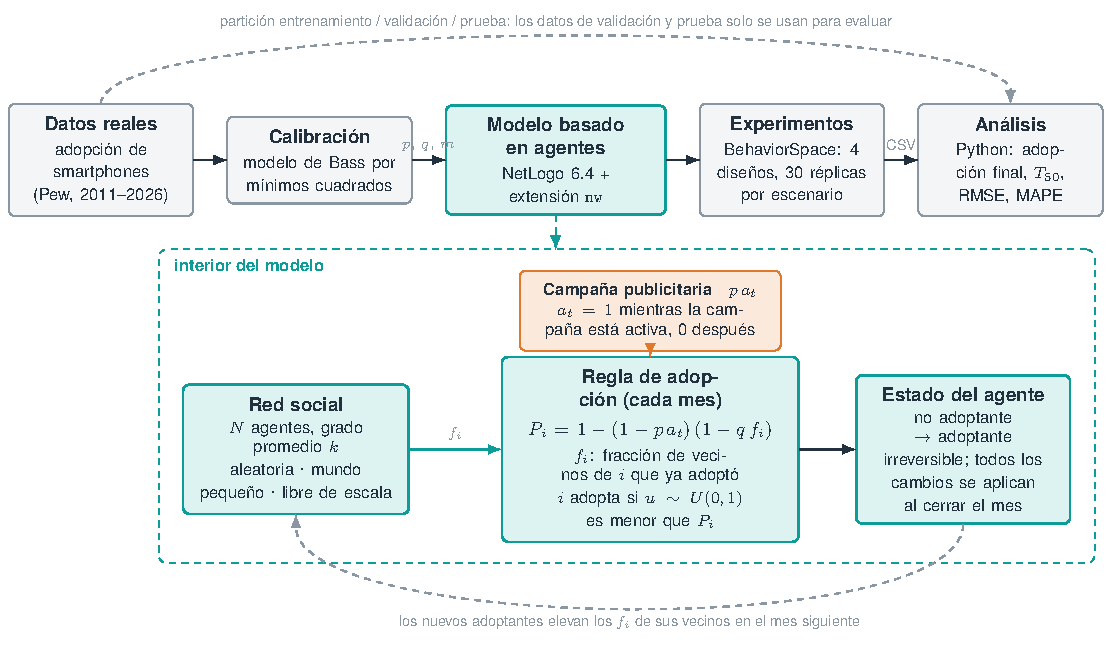
\includegraphics[width=0.94\textwidth]{esquema_sistema.pdf}
  \caption{Esquema del sistema. Arriba, el flujo de trabajo; abajo, el interior del modelo: la red provee la fracción de vecinos adoptantes $f_i$, la campaña la señal $a_t$, y la regla decide el cambio de estado de cada agente.}
  \label{fig:esquema}
\end{figure}

\subsection{Implementación}

El modelo se implementó en NetLogo~\cite{wilensky1999} con la extensión \texttt{nw}, que genera las redes y mide sus propiedades. \texttt{setup} carga los parámetros del caso elegido (PS5, GTA~6 o libre), crea la red, marca el potencial de mercado y siembra los adoptantes iniciales; \texttt{go} ejecuta un mes en dos fases, \texttt{decidir} (cada no adoptante calcula $f_i$ y sortea su decisión) y \texttt{actualizar} (aplica las decisiones a la vez, registra las medidas e integra~\eqref{eq:bass} como referencia).

\subsection{Calibración y analogía}
\label{sec:calibracion}

\textbf{PS5.} Los parámetros de~\eqref{eq:bass} se estimaron por mínimos cuadrados no lineales en la partición de entrenamiento, con $t=0$ en el lanzamiento (12 de noviembre de 2020). Como el potencial $m$ no es identificable desde la fase de crecimiento (el ajuste libre lo lleva a la cota superior), se trató como hiperparámetro: para cada $m$ de una rejilla entre 0,80 y 1,00 se estimaron $p$ y $q$ y se eligió el de menor error en validación; como ese error bajó hasta el tope (la base de la PS4), $m=1$ es un supuesto conservador. Los coeficientes anuales se pasaron a tasas mensuales ($p/12$, $q/12$).

\textbf{GTA~6.} Sin ventas propias, se parametrizó por analogía~\cite{thomas1985} con GTA~V, lanzado en 2013 para PS3 y Xbox 360 (\cifraGtaBase\ millones de consolas instaladas). Sus ventas oficiales llegaron a \cifraGtavSeisSemanas\ millones a las seis semanas y se estabilizaron en \cifraGtavMeseta\ millones al año~\cite{taketwo2014}, el \cifraGtavMesetaPct\,\% de la base. Con la recursión mensual de~\eqref{eq:bass}, $m$ igual a esa meseta, $q$ igual al de la PS5 y 11,2 millones de compradores el primer día\footnote{Guinness World Records (2013), con datos de Rockstar; Take-Two no publicó esa cifra.}, el ajuste da $p=\cifraGtaP$ mensual (error de \cifraGtaRmse\ puntos): con $q$ fijado, el salto del lanzamiento se atribuye a la influencia externa ($p\approx\cifraGtaRazonPQ\,q$), al revés que en la PS5. GTA~6 se modela sobre los dueños de PS5 con $m=\cifraGtaM$\,\%, \cifraGtaIniciales\,\% de compradores el primer día y esos $p$ y $q$.

\section{Conjunto de datos}
\label{sec:datos}

\textbf{Serie real.} La serie principal son las unidades de PS5 vendidas a tiendas que Sony Interactive Entertainment publica por trimestre fiscal~\cite{sony2026}: \cifraTrimestres\ trimestres, desde el de lanzamiento (diciembre de 2020) hasta septiembre de 2026, que van de \cifraPsUnidadesIni\ a \cifraPsUnidadesFin\ millones acumulados. El porcentaje de adopción se expresa sobre la base instalada de la generación anterior, la PS4, con más de \cifraUniverso\ millones de unidades según la misma fuente; ese universo se fijó antes de ver la partición de prueba. La Tabla~\ref{tab:datos} muestra ejemplos. La serie de GTA~V tiene cinco valores acumulados entre septiembre de 2013 y agosto de 2014 (\cifraGtavSerie\ millones): el primero, de Guinness, y los demás, de Take-Two.

\begin{table}[htb]
\centering
\caption{Cinco de los 24 trimestres de la serie real: unidades de PS5 vendidas a tiendas (millones), acumulado y porcentaje de la base de PS4 (117 M).}
\label{tab:datos}
\small
\setlength{\tabcolsep}{4pt}
\begin{tabular}{llrrrl}
\toprule
trimestre & cierre & unidades & acumulado & \% base PS4 & partición \\
\midrule
FY2020~Q3 & 31-dic-2020 & 4,5 & 4,5 & 3,8 & entrenamiento \\
FY2022~Q3 & 31-dic-2022 & 7,1 & 32,1 & 27,4 & entrenamiento \\
FY2024~Q3 & 31-dic-2024 & 9,5 & 75,0 & 64,1 & validación \\
FY2025~Q3 & 31-dic-2025 & 7,9 & 92,2 & 78,8 & prueba \\
FY2026~Q2 & 30-sep-2026 & 2,6 & 97,9 & 83,7 & prueba \\
\bottomrule
\end{tabular}
\end{table}


\textbf{Datos simulados.} Cada experimento exporta una fila por corrida y mes con los parámetros y las medidas: \cifraCorridas\ corridas de 1000 agentes y \cifraFilas\ filas en CSV.

\section{Diseño experimental}
\label{sec:diseno}

\textbf{Partición.} La serie de la PS5 se dividió cronológicamente en entrenamiento, de diciembre de 2020 a diciembre de 2023 (\cifraObsEnt\ trimestres), con el que se estiman $p$ y $q$; validación, de marzo a diciembre de 2024 (\cifraObsVal\ trimestres), con el que se eligen $m$ y la estructura de red; y prueba, de marzo de 2025 a septiembre de 2026 (\cifraObsPru\ trimestres), que no interviene en ninguna decisión. Como control adicional se usa el dato de Sony posterior a la serie: más de 100 millones al 10 de noviembre de 2026 (\cifraControlReal\,\% de la base).

\textbf{Medidas de desempeño.} La principal es el \emph{porcentaje de adopción al final del período}: la fracción de la población que ha adoptado a los \cifraHorizontePs\ meses del lanzamiento en la PS5 y a los \cifraHorizonteGta\ en GTA~6. Se reportan además el mes del 50\,\% y el del pico de adoptantes nuevos. Frente a la serie real, por partición, se usan la raíz del error cuadrático medio (RMSE, en puntos porcentuales) y el error porcentual absoluto medio (MAPE) entre la curva simulada promedio y el valor observado al cierre de cada trimestre. Con 30 réplicas por escenario se reportan medias e intervalos de confianza del 95\,\% ($t$ de Student), que recogen la variabilidad entre réplicas, no la incertidumbre de $p$, $q$ y $m$.

\textbf{Escenarios.} La Tabla~\ref{tab:experimentos} resume los cuatro experimentos. E1 a E3 se corren para ambos casos con $N=1000$ y la red de mundo pequeño con $k=16$, la elegida en validación, salvo en el factor que varía. En la PS5 se siembra un 2,5\,\% de adoptantes iniciales (la categoría de innovadores de Rogers~\cite{rogers2003}) para que el escenario sin campaña pueda arrancar; en GTA~6, los compradores del primer día. Sin campaña, $p=0$ desde el lanzamiento: se suprime toda influencia externa, así que la diferencia entre escenarios es una cota superior del efecto de la publicidad.

\begin{table}[htb]
  \centering
  \caption{Experimentos (30 réplicas por combinación); E1 a E3, para PS5 y GTA~6.}
  \label{tab:experimentos}
  \footnotesize
  \setlength{\tabcolsep}{4pt}
  \begin{tabular}{llr}
    \toprule
    exp. & factores y niveles & corridas \\
    \midrule
    E1 & publicidad \{sin, con\} $\times$ densidad $k\in\{2,4,6,8,12,16\}$ & 720 \\
    E2 & publicidad $\times$ topología \{aleatoria, mundo pequeño, libre de escala\} & 360 \\
    E3 & duración de la campaña \{0, 1, 3, 6, 12, 24 meses, permanente\} & 420 \\
    E4 & calibración (PS5): topología (3) $\times$ $k\in\{4,8,16\}$, 74 meses & 270 \\
    \bottomrule
  \end{tabular}
\end{table}

\textbf{Verificación.} La regla se reimplementó en Python con \texttt{networkx} y se repitieron los cuatro experimentos. En los \cifraVerifEscenarios\ escenarios, la adopción final media difiere en \cifraVerifDifMedia\ puntos en promedio (\cifraVerifDifMax\ como máximo); con la prueba $t$ de Welch, \cifraVerifSignif\ difieren sin corregir, lo esperable por azar, y con la corrección de Holm \cifraVerifHolm. Con la red completa, la regla recupera la recursión de Bass (diferencia máxima de \cifraVerifBassMax\ puntos).

\section{Resultados}
\label{sec:resultados}

\subsection{Calibración y validación con la PS5}

El ajuste en entrenamiento dio $p=\cifraBassP$ y $q=\cifraBassQ$ anuales, con $m=\cifraBassM$\,\% (tope de la rejilla): la imitación pesa \cifraBassRazonQP\ veces más que la publicidad. Con los mismos coeficientes, en las redes la difusión es más lenta que en el modelo agregado, porque parte de la influencia de cada adoptante recae sobre vecinos que ya adoptaron; las nueve estructuras quedan por debajo de la serie y el error baja con $k$ (Tabla~\ref{tab:calibracion}). La validación eligió la \cifraAbmSelRedNombre\ con $k=\cifraAbmSelK$ (\cifraAbmRmseVal\ puntos, frente a \cifraAbmSegundaRmseVal\ de la \cifraAbmSegundaRedNombre\ con $k=\cifraAbmSegundaK$, una diferencia pequeña frente a la variabilidad entre réplicas). Su error en prueba es de \cifraAbmRmsePru\ puntos (MAPE \cifraAbmMapePru\,\%), mayor que el \cifraBassRmsePru\ del modelo agregado. Ambos quedan por debajo del control de noviembre de 2026 (\cifraControlAbm\,\% y \cifraControlBass\,\% frente a más de \cifraControlReal\,\%; Figura~\ref{fig:calibracion}): el ajuste con toda la serie sugiere que la PS5 superará la base de la PS4 (unos \cifraBassMLibreM\ millones).

\begin{table}[tb]
\centering
\caption{RMSE del ABM (puntos porcentuales) frente a la serie real en validación / prueba, por topología y grado promedio. La estructura se elige por el menor RMSE en validación ($\star$); la partición de prueba no interviene en ninguna decisión. El modelo agregado de Bass obtiene 0,63 / 3,10.}
\label{tab:calibracion}
\small
\setlength{\tabcolsep}{4pt}
\begin{tabular}{lrrr}
\toprule
modelo & $k=4$ & $k=8$ & $k=16$ \\
\midrule
ABM aleatoria & 4,90 / 5,37 & 2,68 / 4,04 & 2,50 / 3,99 \\
ABM mundo pequeño & 4,10 / 4,78 & 2,91 / 4,28 & 2,39 / 4,04 \\
ABM libre de escala & 4,68 / 5,14 & 2,65 / 4,02 & 1,93 / 3,74$\star$ \\
\bottomrule
\end{tabular}
\end{table}


\begin{figure}[htb]
  \centering
  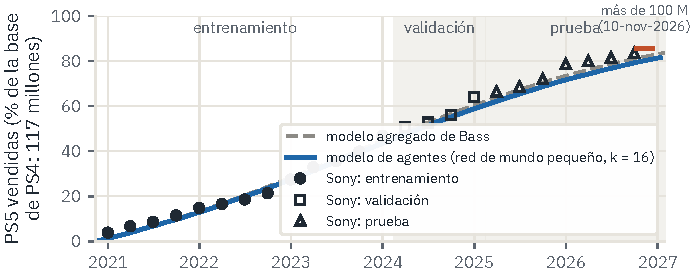
\includegraphics[width=0.8\textwidth]{fig_calibracion.pdf}
  \caption{Serie de la PS5 por partición, curva de Bass ajustada y curva media (banda: IC 95\,\%) del modelo de agentes con la estructura elegida en validación. El trazo horizontal marca el control de Sony del 10 de noviembre de 2026.}
  \label{fig:calibracion}
\end{figure}

\subsection{Publicidad y densidad de la red}

La Figura~\ref{fig:escenarios}(a, b) muestra las curvas de E1 para la red más dispersa y la más densa. En la PS5, sin publicidad la adopción a seis años va del \cifraPsSinKDos\,\% con $k=2$ al \cifraPsSinKDieciseis\,\% con $k=16$ y nunca alcanza el 50\,\%; con campaña la curva toma forma de S, cruza el 50\,\% hacia el mes \cifraTcincuentaPsConKDieciseis\ con $k=16$ y alcanza entre el \cifraPsConMin\,\% y el \cifraPsConMax\,\%. La densidad pesa mucho más, en términos relativos, sin publicidad: pasar de $k=2$ a $k=16$ multiplica la adopción por \cifraPsSinRazon\ (+\cifraPsSinGanancia\ puntos), porque con más contactos la influencia sale antes de los grupos locales; con campaña, solo por \cifraPsConRazon\ (+\cifraPsConGanancia\ puntos), porque la publicidad siembra adoptantes en toda la red. El nivel sin campaña depende de la semilla inicial (\cifraSensSemillaUnoSin\,\% con un 1\,\% de innovadores y \cifraSensSemillaCincoSin\,\% con un 5\,\%), pero sigue lejos del que da la campaña. En GTA~6 la campaña lo decide todo: con ella se alcanza el potencial (entre \cifraGtaConMin\,\% y \cifraGtaConMax\,\%) con el pico de compras en el mes \cifraMesPicoGtaConKDieciseis; sin ella, la adopción apenas pasa de los compradores del primer día (\cifraGtaSinMin\,\% a \cifraGtaSinMax\,\%), cualquiera que sea la densidad.

\begin{figure}[htb]
  \centering
  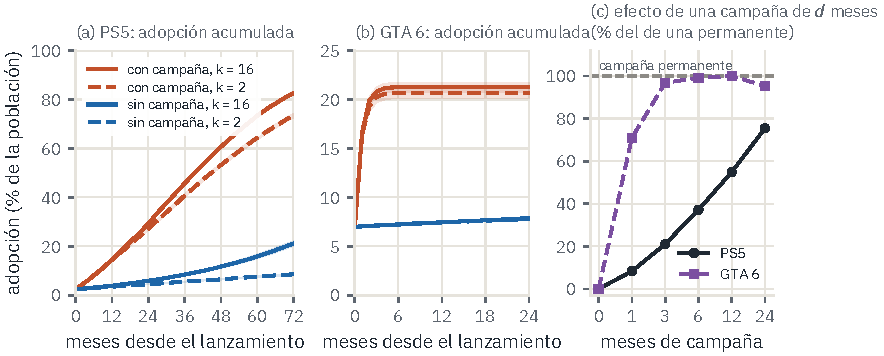
\includegraphics[width=\textwidth]{fig_escenarios.pdf}
  \caption{(a, b) Curvas medias de adopción (banda: IC 95\,\%) con y sin campaña en redes de mundo pequeño con $k=2$ y $k=16$, para la PS5 (a) y GTA~6 (b). (c) Efecto de una campaña de $d$ meses como porcentaje del de una permanente, $(A_d-A_0)/(A_{\text{perm}}-A_0)$; los valores sobre 100\,\% son variación entre réplicas.}
  \label{fig:escenarios}
\end{figure}

\subsection{Topología de la red}

En E2 las tres topologías tienen $k=16$, pero la de mundo pequeño tiene mucho más agrupamiento ($C=\cifraEstMundoC$ frente a \cifraEstAleatoriaC\ en la aleatoria y \cifraEstEscalaC\ en la libre de escala). Con campaña las tres convergen (PS5: \cifraTopoPsConMin\,\% a \cifraTopoPsConMax\,\%). Sin campaña, en la PS5 la de mundo pequeño es la más lenta (\cifraTopoPsSinMundo\,\% frente a \cifraTopoPsSinAleatoria\,\% en la aleatoria y \cifraTopoPsSinEscala\,\% en la libre de escala), porque la influencia se queda en grupos ya convencidos; la libre de escala es la más variable (desviación estándar de \cifraTopoPsSinEscalaDe\ puntos, frente a \cifraTopoPsSinAleatoriaDe\ y \cifraTopoPsSinMundoDe), porque depende de si un nodo muy conectado adopta temprano. En GTA~6 la topología no cambia el resultado.

\subsection{Duración de la campaña}

E3 interrumpe la campaña después de un número dado de meses (Figura~\ref{fig:escenarios}(c)). En GTA~6, un mes de campaña logra el \cifraFraccionGtaDUno\,\% del efecto de una permanente y tres meses el \cifraFraccionGtaDTres\,\%: el lanzamiento concentra casi todo. En la PS5 el rendimiento es gradual: un año de campaña logra el \cifraFraccionPsDDoce\,\% del efecto y dos años el \cifraFraccionPsDVeinticuatro\,\% (\cifraDurPsDVeinticuatro\,\% de adopción frente a \cifraDurPsDPermanente\,\%), porque la imitación necesita tiempo para sostener la difusión.

\section{Conclusiones}
\label{sec:conclusiones}

El modelo sigue la partición de prueba de la PS5 con un error de \cifraAbmRmsePru\ puntos y permite evaluar escenarios contrafactuales. Primero, en una tecnología que se difunde por imitación, como la PS5, la publicidad es la condición del despegue (como máximo \cifraPsSinMaxGlobal\,\% sin campaña en cualquiera de las redes, frente a al menos \cifraPsConMin\,\% con ella) y su efecto se acumula con los meses. Segundo, en un lanzamiento dominado por la influencia externa, como GTA~6, el primer mes de campaña decide el resultado y la red casi no importa. Tercero, la densidad de la red pesa mucho más, en términos relativos, sin publicidad, y la topología solo importa sin ella. Las limitaciones son los coeficientes homogéneos, la red estática, que las unidades vendidas a tiendas no equivalen a compradores y que los parámetros de GTA~6 son hipotéticos (con su potencial y sus compradores del primer día duplicados, el modelo da \cifraSensDobleSin\,\% sin campaña y \cifraSensDobleCon\,\% con ella: cambia el nivel, no el papel de la campaña); además, quitar la campaña suprime toda influencia externa, así que su efecto es una cota superior. Queda contrastar el escenario con las primeras ventas de GTA~6.

\bibliographystyle{splncs04}
\bibliography{referencias}

\end{document}
